\section{Arbres d'attaque et de défense}
	\label{sec:etat_art}

    \subsection{Concept des arbres d'attaque et de défense}
        Le concept des arbres d'attaque a été introduit en 1999 par Bruce Schneier, un expert américain en sécurité informatique qui est parti du constat que des systèmes réputés \og inviolables \fg se font briser en permanence \cite{doc_Schneier}. De plus, ces systèmes sont brisés par des méthodes d'accès qui n'avaient pas été imaginées par leurs concepteurs, car ils n'avaient pas les outils pour dresser une liste exhaustive des attaques possibles. Schneier a donc créé le concept des arbres d'attaque dans ce but : pouvoir réaliser un inventaire complet des méthodes d'attaque sur un système, quel qu'il soit, afin de pouvoir en concevoir la défense de la manière la plus adaptée. Schneier a lui-même conçu son modèle d'arbre d'attaque à partir du principe des \og arbres de défaillances \fg, une méthodologie datant du début des années soixante. Son but est de pouvoir évaluer l'impact de la défaillance d'un composant sur le système dont il fait partie \cite{defaillanceTree}.

        % Utiliser fig:arbre_exemple_1 pour expliquer le formalisme: plus visuel, plus clair
		Lors de ces recherches, Schneier a retenu un formalisme précis : une représentation des menaces sous la forme d'arbres. La Figure \ref{fig:arbre_exemple_1} va servir de support à l'explication de ce formalisme.

        Les arbres sont réalisés en se posant la question suivante : si l'attaquant veux atteindre tel objectif, qu'est ce que cela pré-suppose qu'il accomplisse d'abord ? Pour cela, on représente l'objectif principal (dans notre exemple : acceder au compte en banque d'une personne quelconque) à la racine de l'arbre (en haut), et l'on ajoute en descendant dans l'arbre des nœuds représentant des objectifs intermédiaires à réaliser et qui nous garantissent l'accomplissement de l'objectif principal. Les éléments (nœuds et feuilles) de l'arbre sont traditionnellement représentés par des ronds. 

        L'ajout de ces nœuds peut se faire sous deux formes distinctes : par disjonction ou conjonction. La disjonction correspond à des cas où la validation d'un seul des nœuds enfants valide le nœud parent (opération logique OU, représentée par des traits simples) : par exemple, accéder au compte en banque peut se faire soit par ATM, soit par internet ; une seule des méthodes d'accès suffit. La conjonction quant-à elle correspond à des cas où il faut valider l'ensemble des nœuds enfants pour valider le nœud parent (opération logique ET, représentée par des traits simples reliés entre eux par un arc) : Ainsi pour accéder au compte bancaire de quelqu'un, il faut à la fois son numéro de carte et son code PIN ; la validation d'un seul des deux noeuds enfants n'est pas suffisante pour la validation du noeud parent "accéder compte par ATM". 

        Le formalisme stipule également que si des noeuds enfants doivent être validés dans un ordre précis pour valider le noeud parent, ils seront disposés selon un ordre gauche droite : par exemple, on pourrait considérer que le noeud "obtenir mot de passe" doit être validé avant celui "obtenir login". L'on fait ensuite découler de ces objectifs intermédiaires d'autres objectifs les validant et ainsi de suite, jusqu'à avoir les actions de base aux feuilles de l'arbre (en bas). Ensuite, il suffit de descendre dans l'arbre à partir d'un nœud pour savoir quelles sont les combinaisons d'actions possibles à effectuer pour valider le nœud.

		Lors de ses recherches, Schneier a retenu une représentation des menaces sous la forme d'arbres, expliquée par la Figure \ref{fig:arbre_exemple_1}. Ces arbres modélisent les pré-requis nécessaires à la réalisation de l'objectif principal (dans notre exemple, accéder au compte en banque d'une personne). Pour cela, on représente d'abord ce dernier à la racine de l'arbre, puis on le décompose en objectifs intermédiaires, appelés \og nœuds \fg. Ces derniers sont ensuite re-décomposés de la même façon en répétant l'opération autant que nécessaire. Le dernier objectif de la décomposition est appelé \og feuille \fg. Les différents éléments de l'arbre sont par convention représentés par des ovales. 
	
		\begin{figure}[htbp]
	        %\hspace*{-10cm}
	        \centering
	        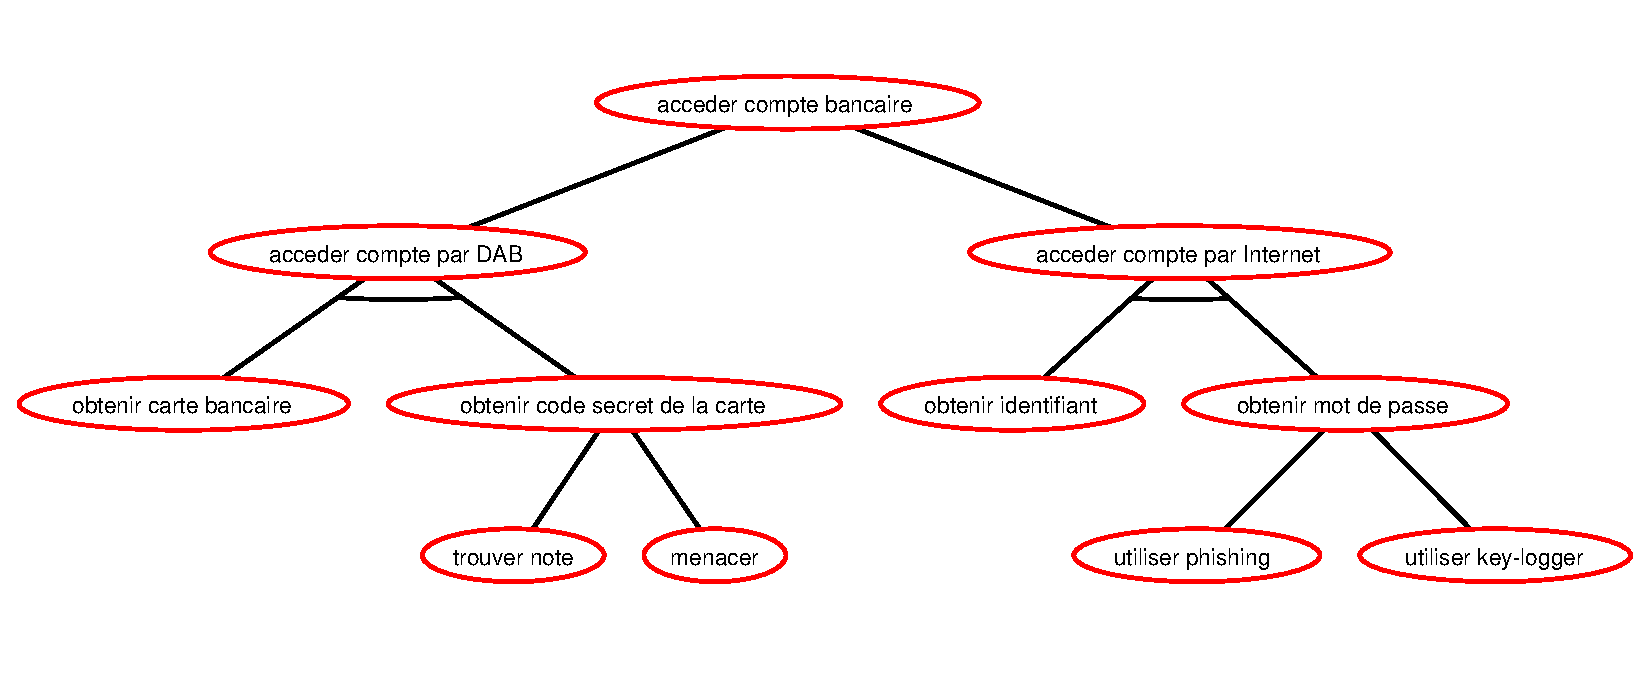
\includegraphics[width=\textwidth]{figure/exemple1_rapport.pdf}%scale=1.2
	        \caption{Arbre d'attaque}
	        \label{fig:arbre_exemple_1}
        \end{figure}

        La relation entre les fils d'un nœud peut prendre deux formes distinctes :
        \begin{itemize}
        \item la {\bf disjonction}, qui correspond au cas où la validation d'un seul nœud fils suffit à valider le nœud père. Ceci équivaut à l'opération logique \og OU \fg{}, et est représenté par des traits pleins. Dans notre exemple, accéder au compte en banque de quelqu'un peut se faire soit par un distributeur de billets (DAB), soit par Internet.
        
        \item la {\bf conjonction}, qui correspond au cas où la validation de l'ensemble des nœuds fils suffit à valider le nœud père. Ceci équivaut à l'opération logique \og ET \fg{}, et est représentée par des traits pleins reliés par un arc. Par exemple, pour accéder au distributeur de billets, il faut à la fois sa carte et son code PIN.
         \end{itemize}

	\paragraph{}
        Enfin, le modèle des arbres d'attaque permet d'associer aux feuilles des valeurs représentant des informations sur l'action : coût, difficulté, probabilité, temps d'exécution, etc. Ces valeurs permettent de quantifier le poids du nœud dans l'arbre. Il est alors possible, à partir de ces données et en utilisant les fonctions appropriées, de les propager au nœud père. Ceci permet à l'attaquant de choisir une stratégie d'attaque plutôt qu'une autre au vu de ses ressources. La Figure \ref{fig:arbre_exemple_2} illustre par exemple le coût monétaire pour l'attaquant. On remarque dans ce cas précis que le coût d'un nœud disjonctif est le coût minimal de ses fils, tandis que le coût d'un nœud conjonctif en est la somme. Chaque quantification a un mode de calcul propre vis-à-vis du types de nœuds (disjonctif ou conjonctif). Il est également possible de combiner plusieurs valuations pour en produire de nouvelles. Par exemple, on peut obtenir la valuation \og risque \fg{}  en multipliant pour l'attaque sa \og probabilité de succès\fg{} par son \og impact\fg{}.

        \begin{figure}[htbp]
	        %\hspace*{-10cm}
	        \centering
	        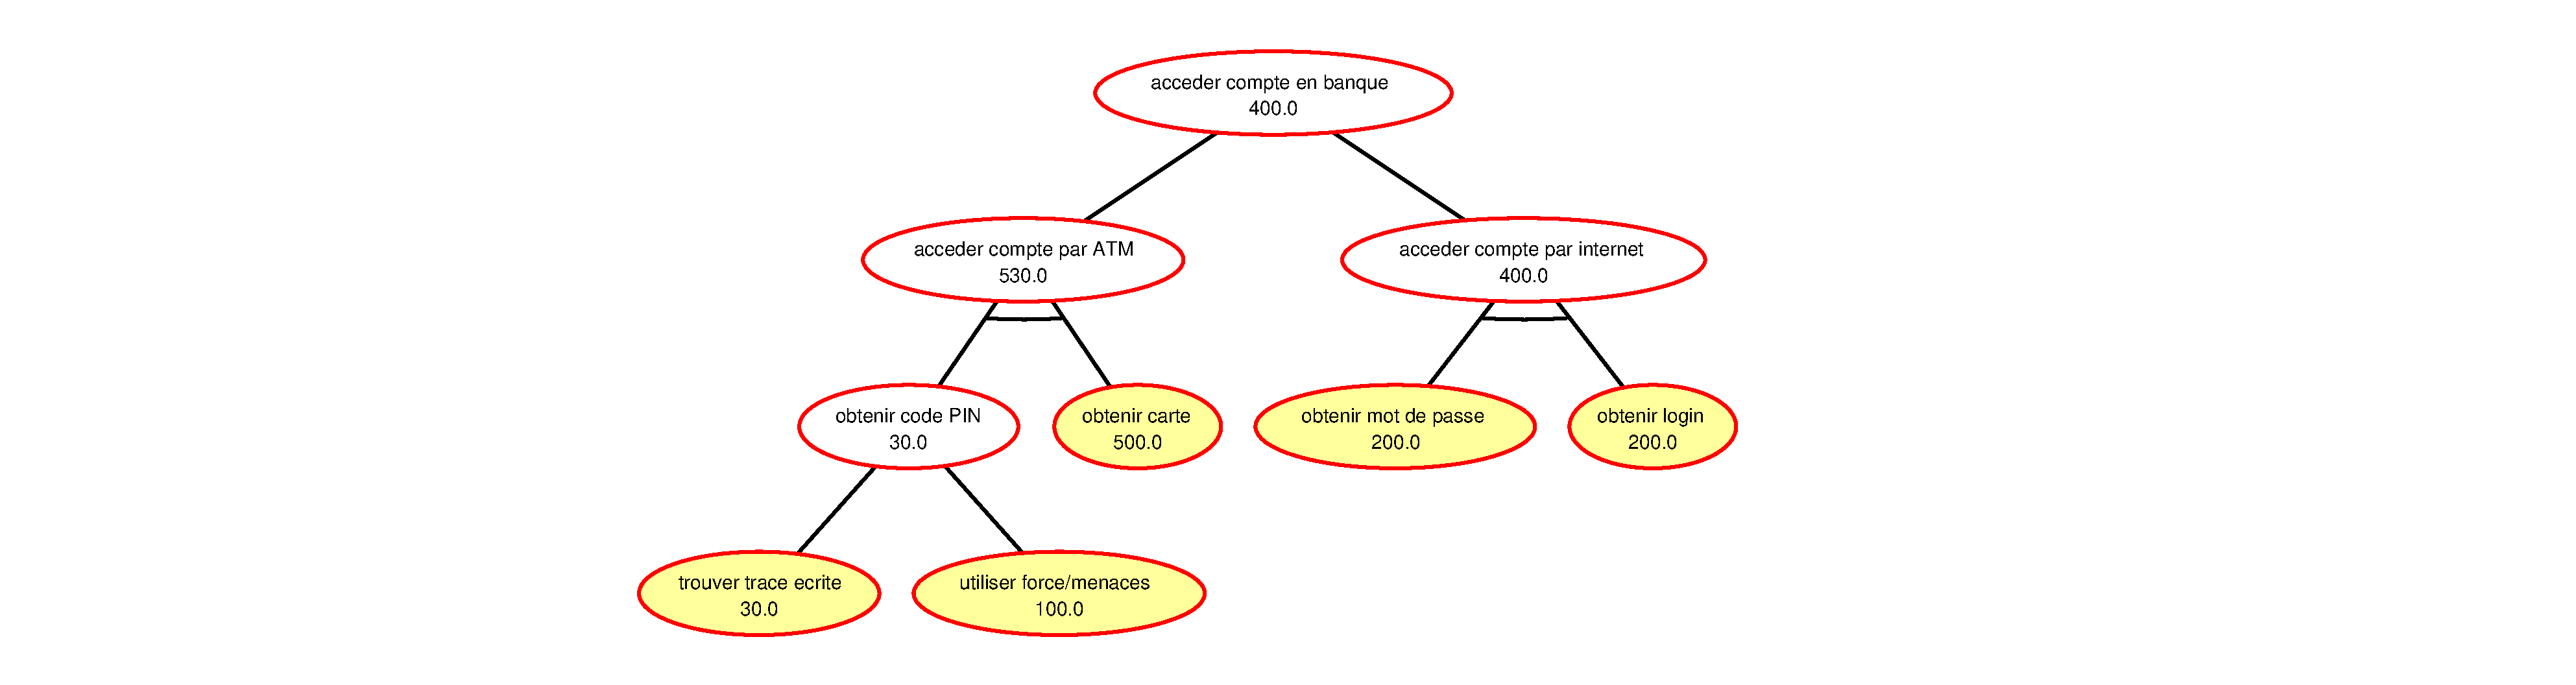
\includegraphics[width=\textwidth]{figure/quantification.pdf}%scale=1.2
	        \caption{Quantification du coût de l'attaque}
	        \label{fig:arbre_exemple_2}
        \end{figure}

		Depuis 1999, le concept des arbres d'attaque a évolué grâce à la contribution de personnes ayant étendu et amélioré le modèle de Schneier \cite{ADTreeKordy}. En particulier, le concept d'arbre d'attaque a été étendu à celui d’arbre d’attaque et de défense (\og attack–defense tree \fg{} en anglais, ou \og ADTree \fg{}). Ce concept amélioré représente également les défenses mises en place que l'attaquant aura besoin de désactiver pour atteindre son but \cite{ADTreeOxford}. Par convention, les défenses sont représentées par des rectangles. La Figure \ref{fig:arbre_exemple_3} représente l'exemple précédent auquel des défenses ont été ajoutées.

        \begin{figure}[htbp]
        	%\hspace*{-10cm}
	        \centering
	        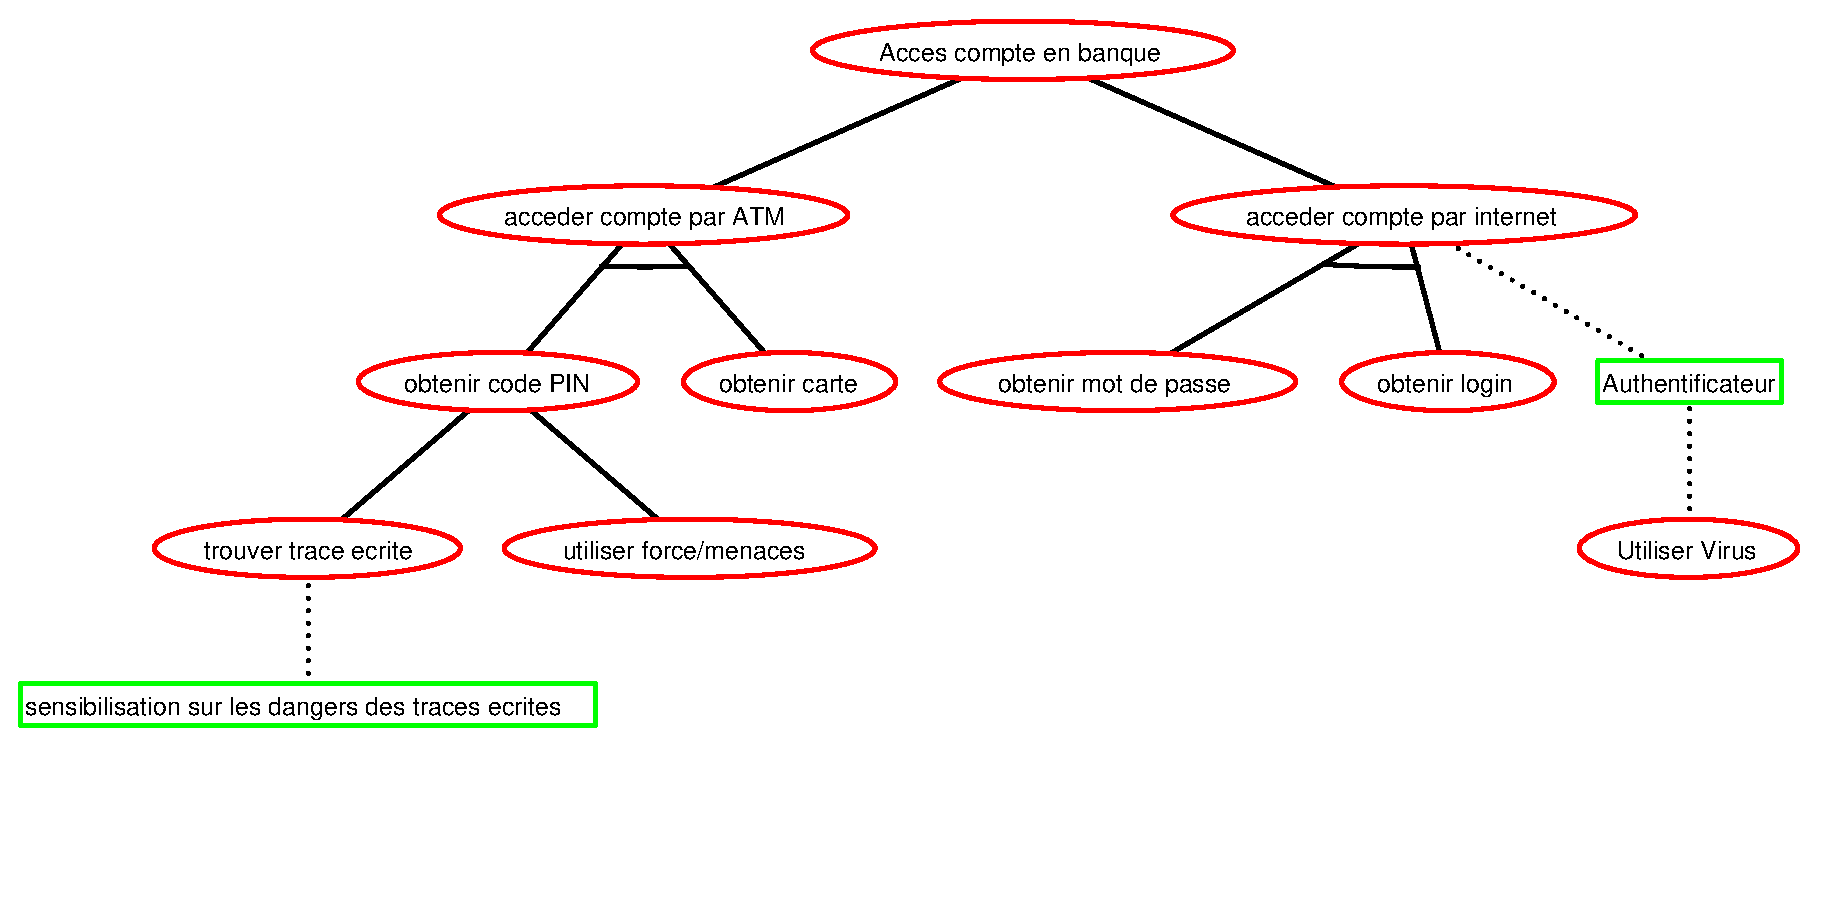
\includegraphics[width=\textwidth]{figure/exemple2_rapport.pdf}%scale=1.2
	        \caption{Implémentation des défenses}
	        \label{fig:arbre_exemple_3}
        \end{figure}

	\subsection{Implémentations des ADTree}
		Plusieurs logiciels implémentant le concept des arbres d'attaque ou des ADTree ont été développés. Quelques-uns sont listés ci-dessous.
        
        Logiciels propriétaires :
        \begin{itemize}
	        \item SecurlTree : Logiciel de création et d'analyse d'arbres d'attaque développé par la société Amenaza \cite{SecurlTree}.
	        \item ATTACKTREE+ : Logiciel de création et d'analyse d'arbres d'attaque développé par la société Isograph \cite{ATTACKTREE+}.
        \end{itemize}
        
        Logiciel Open-Source :
        \begin{itemize}
        	\item ADTool: Logiciel développé par une équipe de chercheur de l'université du Luxembourg pour la modélisation d'ADTrees. Il s'agit d'un des logiciels que nous allons utiliser (plus de détails dans la Section \ref{sec:outils}) \cite{ADTool}.
        \end{itemize}

        \subsubsection{Synthèse}
            Aujourd'hui, les arbres d'attaque sont utilisés par de nombreuses entreprises. Les ADTree présentent l'avantage de pouvoir partir du point de vue de l'attaquant et donc de concentrer les efforts de défenses là où ils seront les plus utiles. Cela dit, un grand nombre de ces entreprises développent en interne leur propre logiciel de construction et d'analyse des ADTree sans toutefois utiliser ceux présents sur le marché. En effet, les solutions logicielles sont rares et ne bénéficient pas d'une grande visibilité, peuvent être chères et ne sont pas forcément faciles à mettre en place. De plus, si il existe tout de même un certain nombre de logiciels implémentant les arbres d'attaques simples, les logiciels implémentant les ADTree sont quant-à eux assez réduits en comparaison. Nous avons pu en identifier un seul : ADTool. 

            Ceci étant, le développement peut être laborieux même en utilisant un logiciel dédié comme ADTool pour plusieurs raisons : le logiciel n’intègre pas d'arbres génériques ce qui rallonge le développement et oblige de modéliser plusieurs fois la même partie d'arbre, ne permet pas de gérer la quantification de manière dynamique selon qui est l'attaquant, etc. Ces limitations seront décrites plus en profondeurs dans la partie suivante.

            Un grand nombre d'améliorations sont donc possibles : ce qui nous amène au cahier des charges.
